\chapter{SSLstrip NTP}

\label{sec:sslstrip-ntp}

\begin{figure}[H]
  \caption{Attaque SSLstrip NTP (diagramme Dia)}
  \fbox{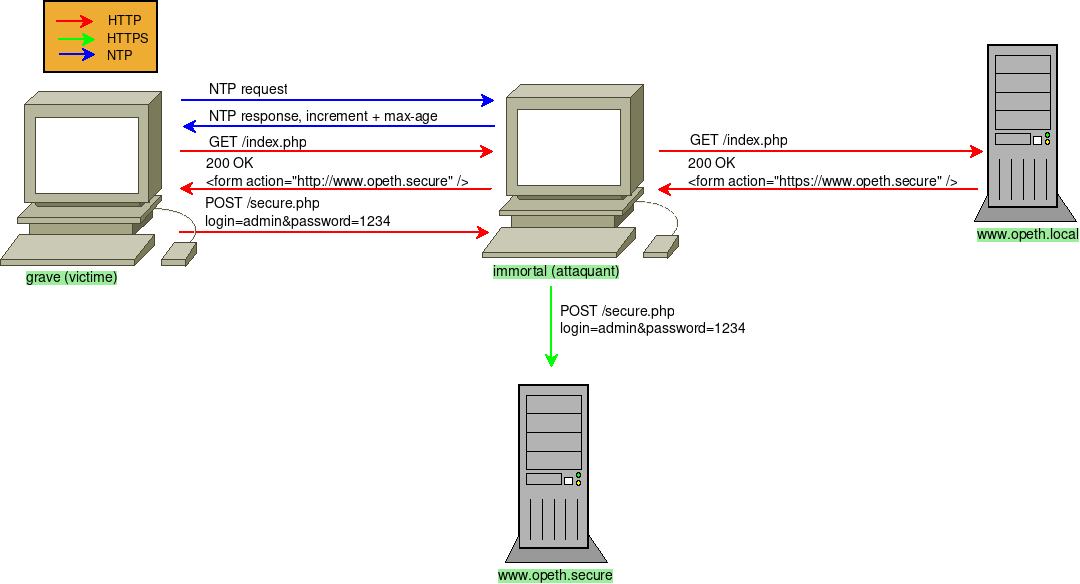
\includegraphics[width=\textwidth]{../medias/sslstrip-ntp/attack.png}}
\end{figure}

\section{Description de l'attaque}

Cette nouvelle amélioration de l'attaque SSLstrip a été présentée lors de la BlackHat Europe par Jose Selvi. Celle-ci utilise le protocole NTP afin de contourner la sécurité offerte par HSTS.

L'attaque SSLstrip originale n'est en effet plus possible lorsque l'on essaye de "striper" les URL d'une page web d'un domaine qui a été protégé ultérieurement par HTTP Strict Transport Security. Le mécanisme HSTS va obliger le client à se connecter à l'URL que l'on cherche à striper en HTTPS pendant un certain laps de temps (défini par le serveur), rendant l'attaque complétement inefficace.

Le protocole NTP (Network Time Protocol) permet de synchroniser l'horloge d'un équipement informatique avec un serveur NTP. Il s'agit d'un protocole stateless basé sur UDP et absolument pas sécurisé. L'attaque présentée par Jose Selvi consiste à usurper les requêtes NTP pour renvoyer une date éronnée au client, et ainsi faire expirer les entrées HSTS. Pour réaliser cela, l'auteur se base sur un outil Python appelé Delorean, qui se comporte comme un serveur NTP et pour lequel on peut définir la date de réponse.

Une fois que l'horloge du client a été compromise et le HSTS du domaine expiré, il est possible d'utiliser l'attaque SSLstrip originale afin de striper les URL des pages web, même pour les domaines censés être protégés par HSTS.

\section{Notre attaque}

Dans ce projet de TER, nous avons eu à réaliser un Proof-Of-Concept de cette attaque. Voici les détails de notre implémentation.

\subsection{Mise en place de l'environnement}

L'environnement de test utilise l'outil Qemunet et est constitué de trois machines virtuelles. Nous avons la machine cliente et victime nommée grave. Ensuite, immortal, la machine de l'attaquant et positionnée en homme du milieu. Finalement, la machine opeth joue le rôle de serveur web hébergeant les deux domaines \path{www.opeth.local} et \path{www.opeth.secure}. Cette dernière machine joue également le rôle du serveur NTP, même si dans la réalité les deux serveurs se trouvent généralement sur des machines différentes.

Pour configurer chaque machine, nous utilisons le script \path{start.sh} présent dans le dossier de chaque machine virtuelle. Ce fichier est lancé au démarrage et permet de configurer les différents services pour la démonstration.

\subsubsection{Machine grave (147.210.13.2)}

Il s'agit de la machine cliente et victime. Celle-ci machine utilise l'environnement graphique de la distribution Linux Alpine et le navigateur firefox est utilisé pour la démonstration.

Au lancement de la machine, le certificat de notre autorité de certification est ajouté à firefox grâce à l'outil certutil. De plus, un client NTP (sntpc) est lancé au démarrage de la machine et configuré pour effectuer ses requêtes vers opeth de manière régulière (toutes les secondes pour les besoins de la démonstration).

\subsubsection{Machine opeth (147.210.12.1)}

Cette machine héberge un serveur HTTP(s) Nginx sur le port 80 et 443. Le certificat utilisé pour les connections HTTPS a été généré avec openssl grâces aux scripts présents dans le dossier \path{CA}, et signé par notre autorité de certification par ce script :

\begin{minted}{bash}
#!/bin/sh

if test ! -f root-ca.pem || test ! -f root-ca.key
then
    echo "[-] First, create CA !"
    exit 1
fi

# Create private key
openssl genrsa -out cert.key 4096

# Create request
openssl req -new -key cert.key -out cert.csr

# Sign certificate with CA
openssl x509 -req -in cert.csr -CA root-ca.pem -CAkey root-ca.key -CAcreateserial -out cert.pem -days 365 -sha256

echo "[+] Your certificate: cert.pem"
echo "[+] Your private key: cert.key"
\end{minted}

Sur le serveur Nginx, nous avons configuré un domaine en http (\path{www.opeth.local}), ainsi qu'un domaine en https (\path{www.opeth.secure}), sécurisé grâce à HSTS. La configuration de ce dernier se fait en rajoutant la ligne suivante dans le fichier de configuration de Nginx :

\begin{minted}{text}
  add_header Strict-Transport-Security "max-age=31536000; includeSubDomains";
\end{minted}

Cette machine héberge également un serveur NTP. Nous avons simplement eu à installer le paquet ntpd pour que celui-ci soit lancé au démarrage.

\subsubsection{Machine immortal (147.210.12.2 - 147.210.13.1)}

C'est sur cette machine que se trouve le Proof-Of-Concept de l'attaque. Nous avons également utilisé le script Delorean comme décrit dans le papier de l'attaque afin d'usurper les requêtes NTP de la machine grave. L'attaque se lance grâce au script \path{/mnt/host/attack.sh} :

\begin{minted}{bash}
#!/bin/sh

PROXY_PORT=4242
DELOREAN_PORT=4343

iptables -t nat -F
iptables -t nat -A PREROUTING -p tcp --destination-port 80 -j REDIRECT --to-port $PROXY_PORT
iptables -t nat -A PREROUTING -p udp --destination-port 123 -j REDIRECT --to-port $DELOREAN_PORT

hsts_expire=$(curl -v https://www.opeth.secure --insecure 2>&1  | grep Strict | awk -F= '{print $2}' | awk -F\; '{print $1}')
hsts_expire=$(($hsts_expire / 60 + 1))

/mnt/host/delorean.py -p $DELOREAN_PORT -n -s ${hsts_expire}m &
/mnt/host/sslstrip-ntp.py $PROXY_PORT
\end{minted}

Nous commençons par rediriger les requêtes HTTP sur le port de notre proxy, puis les requêtes NTP vers le port de Delorean. Nous calculons ensuite le temps d'expiration des entrées HSTS à l'aide de l'outil curl. Finalement, nous lançons le serveur Delorean ainsi que notre proxy implémentant l'attaque SSLstrip.

\subsection{Démonstration}

Dans cette partie, nous allons illustrer l'attaque SSLstrip NTP dans l'environnement que nous avons mis en place. Pour lancer l'environnement de test, il faut lancer la commande suivante (on aura récupéré au préalable le dépôt \textbf{qemunet}) :

\begin{minted}{bash}
./qemunet/qemunet.sh -x -S sslstrip-ntp
\end{minted}

À partir de là, les trois machines sont lancées.

\subsubsection{Étape 1 : avant l'attaque}

Lorsque l'attaque n'est pas encore lancée, nous pouvons voir sur la machine grave que tout se passe normalement et que la requête POST passe bien en HTTPS ; immortal est donc incapable de voir les identifiants envoyés :

\begin{figure}[H]
  \caption{Attaque SSLstrip NTP (avant l'attaque)}
  \fbox{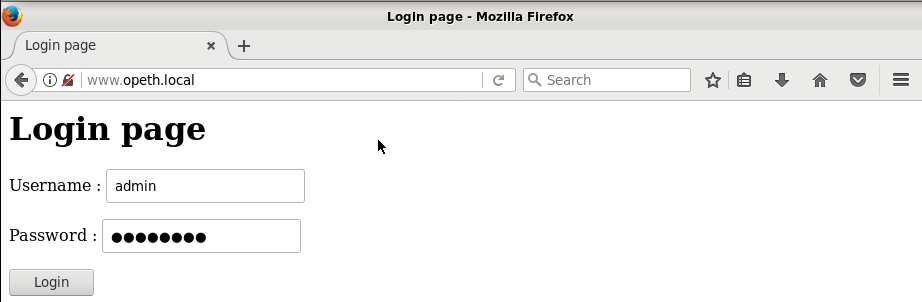
\includegraphics[width=\textwidth]{../medias/sslstrip-ntp/screen1.png}}
\end{figure}


L'encadré rouge ci-dessous montre bien que le POST est effectué en HTTPS, sur le domaine \path{www.opeth.secure}. Lorsque nous affichons le code source de la page, nous obtenons :

\begin{figure}[H]
  \caption{Code source de la page (avant l'attaque)}
  \fbox{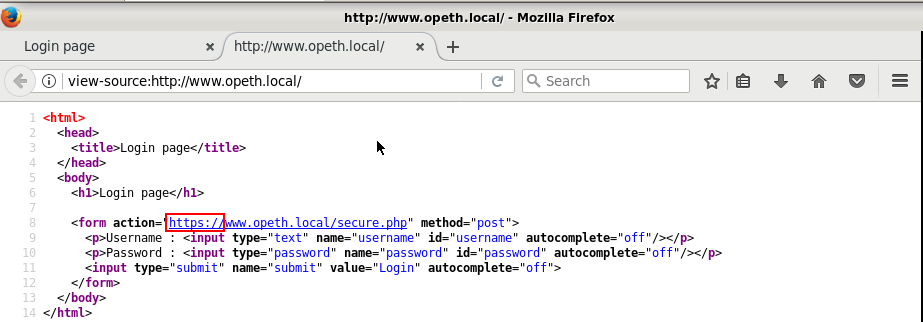
\includegraphics[width=\textwidth]{../medias/sslstrip-ntp/screen2.png}}
\end{figure}

Nous arrivons alors sur le domaine \path{www.opeth.secure} en HTTPS : immortal n'a pas pût voir nos échanges sur cette page sécurisée comme le montre la figure ci-dessous.

\begin{figure}[H]
  \caption{Code source de la page (avant l'attaque)}
  \fbox{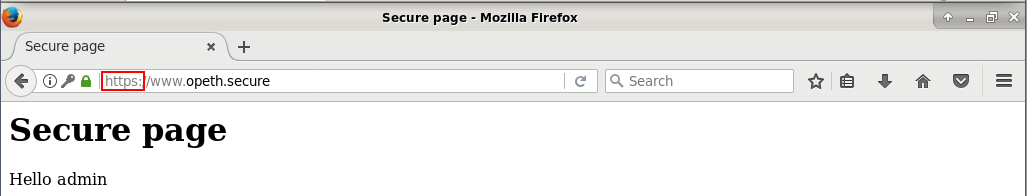
\includegraphics[width=\textwidth]{../medias/sslstrip-ntp/screen3.png}}
\end{figure}

\subsubsection{Etape 2 : pendant l'attaque}

Lorsque l'attaque est en cours et quand le client réalisera une requête NTP, celle-ci va être redirigée vers Delorean qui répondra avec une date permettant de faire expirer son entrée HSTS. Ensuite, quand la machine grave visitera la page non-sécurisée \path{www.opeth.local}, tous les liens HTTPS vers \path{www.opeth.secure} seront strippés.

Ici on voit dans le code source de la page que notre proxy a remplacé les liens \path{https://} par \path{http://}.

\begin{figure}[H]
  \caption{Code source de la page (pendant l'attaque)}
  \fbox{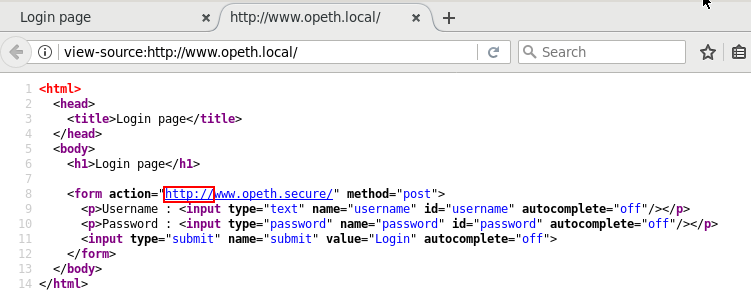
\includegraphics[width=\textwidth]{../medias/sslstrip-ntp/screen5.png}}
\end{figure}

Nous constatons que nous arrivons sur le domaine www.opeth.secure en HTTP : notre navigation n'est pas sécurisée !

\begin{figure}[H]
  \fbox{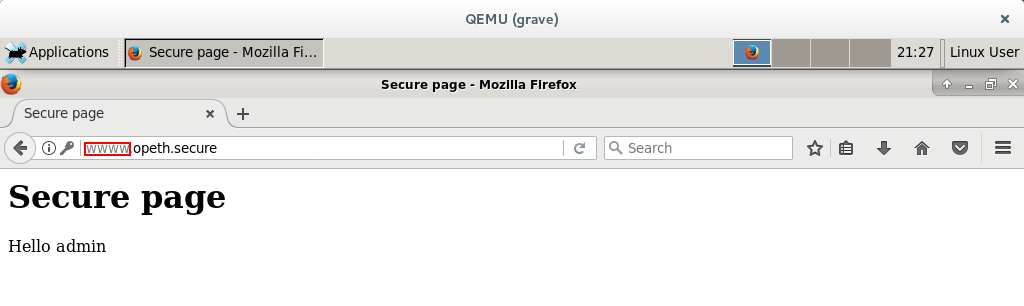
\includegraphics[width=\textwidth]{../medias/sslstrip-ntp/screen6.png}}
\end{figure}

La machine immortal a été capable de capturer non seulement les identifiants du formulaire, mais également le cookie de session alors que le domaine était protégé par HSTS :

\begin{figure}[H]
  \fbox{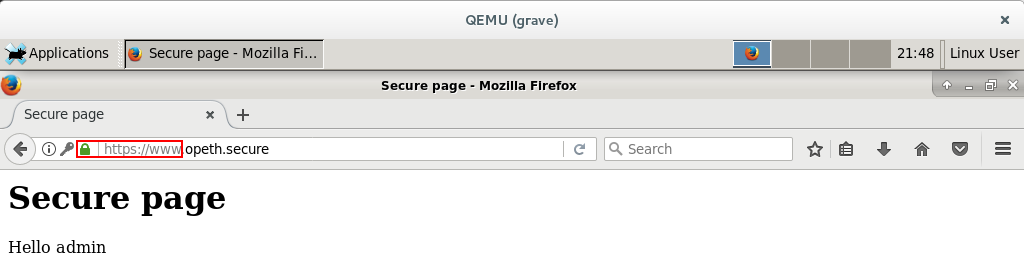
\includegraphics[width=\textwidth]{../medias/sslstrip-ntp/screen7.png}}
\end{figure}

